\section{Experiment and Analysis}

\subsection{Experiment Design}

\paragraph{The Goal}

To test if the model could realistically simulate the buoyancy force, an experimental simulation immitating the scenario introduced at the beginning of the article where a plank falls into the water is setup.
There are two aspects with which we can judge whether the model is succesful or not:
\begin{enumerate}
	\item Will the plank float back to the water surface and oscillate up and down until it reaches a stable state?
	\item Will the plank turn its flat face up under the influence of the buoyancy force?
\end{enumerate}
If all of them are accomplished, we then can say that the model has achieved its goal.

\paragraph{Hardware Information}

The simulation is setup with the Unity engine (version 2022.3.29f1) running on a PC on Windows 11.
The device runs on a CPU of 13th Gen Intel(R) Core(TM) i9-13900HX at 2.20 GHz with 16.0 GB of RAM.

\paragraph{Environment Setup}

In a Unity scene, a block of static water is placed amid the empty space.
A piece of plank is put above the water surface for a couple of meter's height (figure \ref{simulation-environment}).
The plank's density is made to be lighter than the water density so that it floats.
The water block is wide and deep enough so that the plank would never touch the other faces except the top face.

\begin{figure}[h]
	\centering
	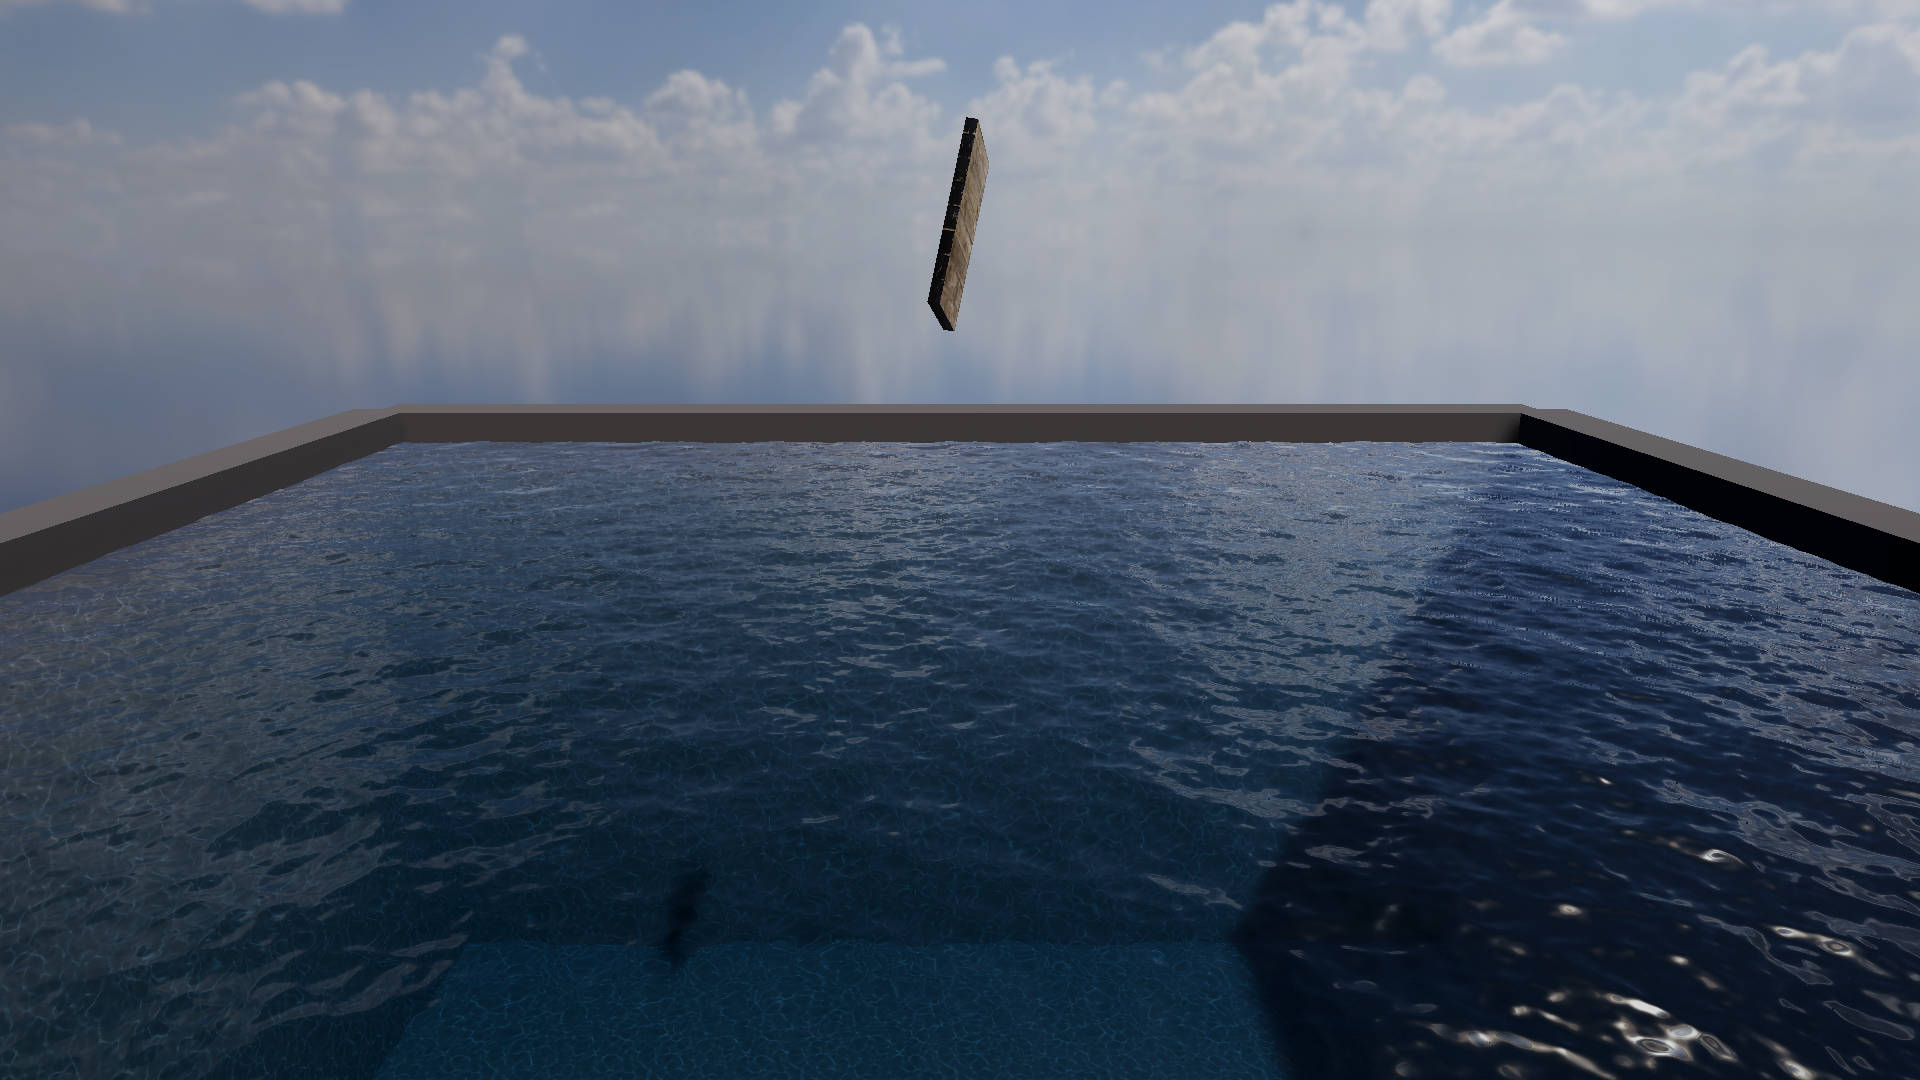
\includegraphics[height=2.5in]{figures/experiment-environment.jpg}
	\caption{The simulation environment.}
	\label{simulation-environment}
\end{figure}

The properties of the water is given in table \ref{simulation-water-properties}.

\begin{table}[h]
	\centering
	\begin{tabular}{ c c c c }
		\hline
		$\rho$ {\footnotesize(density)} & $c_f$ {\footnotesize(form drag coef.)} & $c_v$ {\footnotesize(visc. drag coef.)} & {\small dissipation coef.} \\
		\hline
		1.33 & 0.1 & 0.1 & 1.0 \\
		\hline
	\end{tabular}
	\caption{The properties of the water used in the simulation.}
	\label{simulation-water-properties}
\end{table}

The sampling rate is set at 200 samples per physical frame.

\paragraph{The Process}

At the beginning of the simulation, the plank is let go free-falling into the water.

During the whole process of the simulation, the critical physical properties of the plank will be recorded in every frame for later analysis.

The simulation will stop at an appropriate time after a relatively stable state is reached.

\subsection{Result and Analysis}

The result of a simulation run is shown in the below two figures.

Figure \ref{simulation-result-heights} shows the position of the plank relative to the water surface during the fall.
The olive-colored line shows the position of the plank's center-of-mass, while the blue line shows the height of the lowest point on the plank.

\begin{figure}[htb]
	\centering
	\fbox{
		\begin{tikzpicture}
			\begin{axis}[
				width=5in, height=3in,
				enlargelimits=false,
				xlabel={time (seconds)},
				ymin=-2, ymax=5, ytick={-2,-1,...,5},
			]
				\addplot[black] coordinates { (0,0) (5,0) };
				\addplot[color=olive] table[x=t, y=com] {figures/simulation-record.dat};
				\addplot[color=blue] table[x=t, y=min] {figures/simulation-record.dat};
			\end{axis}
			\matrix [draw, below left] at (4.25in, 2.25in) {
				\node[olive, font=\footnotesize] {center-of-mass}; \\
				\node[blue, font=\footnotesize] {lowest point}; \\
			};
		\end{tikzpicture}
	}
	\caption{The position of the plank during the fall.}
	\label{simulation-result-heights}
\end{figure}

Figure \ref{simulation-result-rot} shows the pitch angle of the plank during the fall.

\begin{figure}[htb]
	\centering
	\fbox{
		\begin{tikzpicture}
			\begin{axis}[
				width=5in, height=2in,
				enlargelimits=false,
				xlabel={time (seconds)},
				ylabel={pitch (degree)},
				ymin=0, ymax=90, ytick={0,15,...,90},
			]
				\addplot[color=red] table[x=t, y=rx] {figures/simulation-record.dat};
			\end{axis}
		\end{tikzpicture}
	}
	\caption{The rotation of the plank during the fall.}
	\label{simulation-result-rot}
\end{figure}

From the figures we can see, soon as the plank touches the water surface (the blue line intersects with the black horizontal line), it immediately started to rotate (the red line rises) so that its flat face is splatted onto the water surface;
meanwhile it started perceiving an upward buoyancy force, repulsing it from continuing falling (the olive line starts accelerating upwards).
Eventually, the plank floats up to the water surface and oscillates to a stable state (the olive line tends to be horizontal);
also, the plank's flat face is aligned to the water surface (red line approaches $y=90$).

Based on the analysis of the result, we can say that our model has met the desired experiment result and is indeed succesful.